\chapter{Architettura interna}

In questo capitolo illustriamo l'architettura interna dell'Engine, cioè del
componente software predisposto alla messa in esecuzione dei programmi Blite.

Ricordiamo che nello scenario delineato avremo un Engine per locazione, o se si
vuole per nodo di rete, e su ognuno di questi componenti sarà possibile
installare o rimuovere definizioni di processi Blite. In pratica un engine
gestir\`a un insieme di definizioni, creando da queste istanze di
processi e utilizzerà l'Environment per interagire con gli altri Engine. 
Dall'environment stesso l'engine verrà notificato riguardo l'accadere di
eventi, quali l'arrivo di messaggi indirizzati alle porte delle sue definizioni.

Dal punto di vista logico relazionale abbiamo già individuato le seguenti
macro entità e relazioni

\begin{figure}[!htp]
\begin{center}
  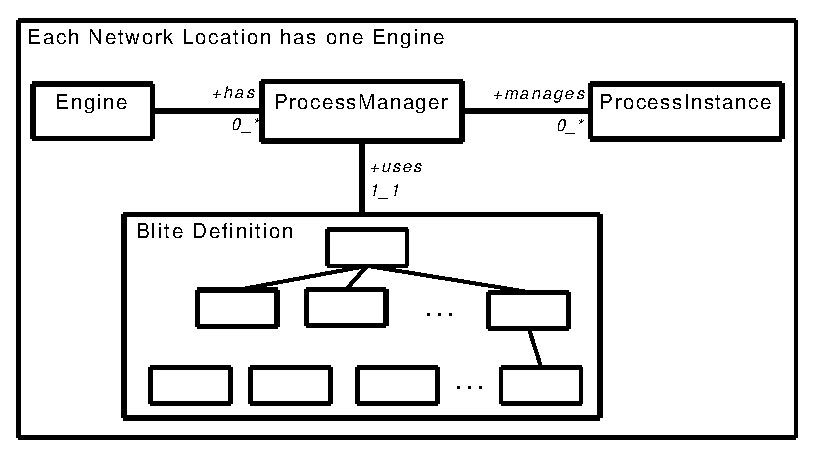
\includegraphics{architettura_interna/dia/engine}
%   \caption[]{
%   	\textsf{{\small Passaggio da reazioni a processi}}
%   }
  \label{fig:1}
\end{center}
\end{figure}

Per ogni definizione istallata sull'engine sarà presente un oggetto istanza
della classe \icode{ProcessManager}, che avrà il compito di gestire, nel loro
ciclo di vita, le istanze di processo derivate dalla definizione.

Prima di entrare nel dettaglio delle scelte architetturali ricapitoliamo quali
sono le caratteristiche peculiari di un sistema che deve gestire programmi per
l'orchestrazione di servizi, in modo che sia pi\`u facile da una parte
comprendere e dall'altra giustificare le scelte fatte.

A nostro vantaggio:
\begin{itemize}
  \item Un Engine contiene in generale un numero contenuto di definizioni, per
  cui non ci interessa la scalabilità rispetto alla quantità di definizioni
  istallate su singolo engine. Tale scalabilità al contrario può essere
  ottenuta aggiungendo altri engine e installando definizioni su engine diversi.
  
  \item  Una definizione (o programma) Blite avendo principalmente funzionalità
  di integrazione avrà una lunghezza generalmente limitata. 
  
  \item Poiché le operazione fondamentali di un programma di questo genere
  sono invocazioni remote, le durate delle esecuzioni hanno ordini di grandezza
  minimi dettati dai tempi caratteristici della rete. Per questo motivo non
  risulta determinante l'efficienza di esecuzione delle operazioni interne di un
  processo. Il nostro engine non necessiterà di una particolare ottimizzazione 
  rispetto all'efficienza di esecuzione interna.
\end{itemize}

al contrario risultano particolarmente critici i seguenti aspetti:
\begin{itemize}
  \item Per ciascuna definizione potrà essere richiesta la creazione di
  innumerevoli istanze. La scalabilità rispetto al numero delle
  richieste remote e quindi di istanze di processo risulta essere un
  prerequisito fondamentale.
  
  \item Se da un lato abbiamo detto che l'efficienza di esecuzione non \`e 
  una aspetto particolarmente critico, dall'altro per\`o ogni attività interna
  necessita di un elevato grado di controllo e tranciabilità. Ogni attività deve
  potere essere eventualmente terminata o abortita. Poiché in generale
  \footnotetext{} ogni istanza potrebbe avere un immagine persistente o
  perlomeno essere soggetta ad una attività di monitoring, l'engine necessiterà
  di un grado di controllo a livello di singola attività Blite.
\end{itemize}

Tenendo conto di queste iniziali considerazioni sono state fatte alcune scelte
basilari di organizzazione del progetto e l'architettura software \`e stata
basata sulle seguenti specifiche fondamentali:

\begin{enumerate}
  \item La compilazione di una definizione Blite (che eventualmente in un
  ambiente distribuito può essere fatta in fase di deploy) produce un modello
  statico della definizione stessa. Tale modello può essere implementato con una
  struttura ad oggetti che si può pensare di mantenere in memoria presso
  l'engine, tale struttura sarà navigata a runtime per ricavare il
  flusso e la logica di esecuzione. Sempre in fase di deploy l'engine può
  ricavare tutte le informazioni per popolare le strutture dati in cui sono 
  memorizzati i binding fra i nomi delle porte e le definizioni; anche tali
  strutture dati possono essere mantenute in memoria.
  
  \item Le richieste che giungono all'Engine non devono produrre un aumento
  delle risorse complessive mantenute dall'Engine. Ogni istanza di processo nel
  suo svolgersi deve, man mano che procede, rilasciare le risorse di memoria
  acquisite. Anche il numero dei thread complessivo deve essere limitato
  superiormente (generalmente dell'ordine dell'unita). La realizzazione del
  parallelismo di attività deve essere attuata tramite il pattern ``Resources
  Pool''. Ogni Engine deve disporre di un pool di thread con cui eseguire in
  parallelo le attività secondo le definizioni Blite.
  
  \item Il modello di esecuzione deve essere Activity Centric. L'engine deve
  trattare ogni attività secondo una astrazione generica che possa permettere di
  fattorizzare i comportamenti comuni e mantenere semplice e pulita
  l'implementazione della semantica di esecuzione del linguaggio.
\end{enumerate}

\section{Modello per l'Attività}
A questo punto dopo aver esposto a grandi linee quelle che devono essere le
caratteristiche fondamentali di un engine entriamo nel dettaglio del disegno
della architettura. Nella realizzazione di questa abbiamo scelto di utilizzare
il formalismo degli oggetti e delle classi secondo il consueto paradigma
``Object Oriented''. Inoltre abbiamo preso come fonte di
ispirazione il ``Composite Pattern'' [GANGo4] cercandone una trasposizione nella
problematica dell'esecuzione di un programma Blite. In particolare
l'astrazione di componente \`e stata applicata all'entità attività. Come i
componenti contribuiscono alla realizzazione di un documento o di una
interfaccia utente le singole attività contribuiscono allo svolgersi
dell'esecuzione del processo Blite.
 
Inoltre la tipica struttura gerarchica presente staticamente negli elementi
sintattici di una definizione può essere naturalmente riprodotta a runtime tra
i singoli step di esecuzione, andato a completare l'analogia con le strutture
gerarchiche ad albero tipiche dei tradizionali domini di applicazione del
Composite Pattern. 
\\

L'entità fondamentale del nostro dominio applicativo \`e stata quindi
individuata nella \icode{ActivityComponent} trasposizione a runtime
dell'elemento sintattico Activity definito dalla grammatica di Blite.
Ogni \icode{ActivityComponent} \`e rappresentabile tramite la seguente
interfaccia

\lstinputlisting
[caption={L'interfaccia base del modello di escuzione del Blite Engine},
label=lst:ActivityComponent]
{architettura_interna/java/ActivityComponent.java}

\begin{tabular}{| p{0.3\textwidth } | p{0.6\textwidth}|}
\hline
\icode{ActivityComponent} &  \\
\hline

\small{boolean \textbf{doActivity()}} & \small{\textsf{Costituisce il metodo
centrale per lo svolgersi dell'esecuzione del programma. L'invocazione di tale metodo su
un oggetto attività fa si che essa possa eseguirsi. Il valore booleano
ritornato sarà il discriminate del fatto che il flusso di esecuzione
corrente dovrà o meno interrompersi. Ogni attività oltre che eseguire se
stesa sarà quindi anche responsabile nel guidare il flusso nel passo
successivo. Utilizzando la gerarchia a lei nota imposterà la nuova attività
corrente da eseguire (l'attività padre o un figlio) e ritornerà il valore true. 
Al contraio potrà interrompere il flusso corrente ritornando false.
}}\\
 
& \\
\small{ActivityComponent \linebreak \textbf{getParentComponent()}} &
\small{\textsf{ Tale metodo restituisce se presente l'elemento padre 
dell'attività corrente. In questo modo si realizza la struttura gerarchica fra
i veri componenti dell'esecuzione. }}\\

& \\
\small{BltDefBaseNode \linebreak {\textbf{ getBltDefNode()}}} &
\small{\textsf{ Ogni attività componente dell'esecuzione \`e strettamente associata ad un 
elemento sintattico del programma. Con questo metodo ogni oggetto attività 
restituisce il nodo che la definisce nell'albero sintattico ricavato dal
parsing del codice Blite. }}\\

\hline
\end{tabular}


Lo scenario che si va a delineare \`e quindi quello di due strutture gerarchiche
associate: una costituita dall'AST (Abstract Syntax Tree) ricavato dal
parsing del codice Blite, e che come si detto \`e mantenuta nella sua interezza,
l'altra costituita dall'albero dinamico delle ActivityComponent che
realizzano l'esecuzione a runtime. Quest'ultima struttura, una per ogni
istanza, non \`e pero costruita in un unico momento in fase di inizializzazione
del  processo, ma al contrario \`e istanziata man mano che l'esecuzione
procede.  Come già accennato le attività stesse saranno responsabili di creare
i loro successori e di metterli in esecuzione. Inoltre gli oggetti attività
già eseguiti dovranno essere rilasciati il prima possibile in modo da poter 
essere collezionati dal Garbage Collector e rilasciare le risorse di memoria.

\begin{figure}[!htp]
\begin{center}
  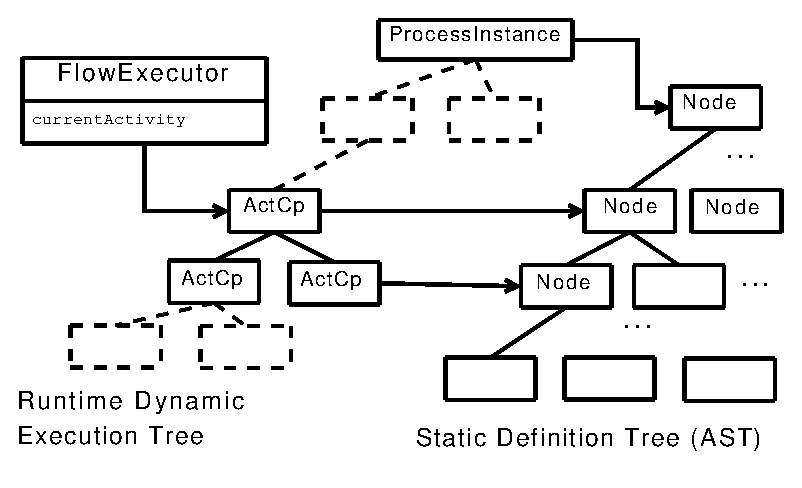
\includegraphics{architettura_interna/dia/tries}
%   \caption[]{
%   	\textsf{{\small Passaggio da reazioni a processi}}
%   }riscrivera
  \label{fig:1}
\end{center}
\end{figure}

Per ogni tipologia di attività prevista dalla grammatica di Blite esisterà
una sotto classe specifica implementante l'interfaccia \icode{ActivityComponent}
e che realizzerà in maniera opportuna in rispetto della semantica il metodo
\icode{boolean \textbf{doActivity()}}. Per ottimizzare il disegno e fattorizzare
il codice comune \`e stata ovviamente introdotta una classe astratta
\icode{ActivityComponentBase} da cui ogni altra implementazione di
\icode{ActivityComponent} erediterà le funzionalità comuni di base.

Anche la classe \icode{ProcessInstance}, che modellerà con i suoi oggetti le
varie istanze di processo nell'engine, implemetra l'interfaccia
\icode{ActivityComponent} uniformando la struttura gerarchica di esecuzione.

Le varie instanze di \icode{ActivityComponent} del tipo specializzato verranno
create tramite una classe di Factory \icode{ActivityComponentFactory} che
espone il FactotyMathod \icode{ActivityComponent
\textbf{makeRuntimeActivity}(BltDefBaseNode bltDefNode,\ldots )} 

\lstinputlisting
[caption={ActivityComponentFactory la factory per le ActivityComponent}
label=lst:ActivityComponentFactory]
{architettura_interna/java/ActivityComponentFactory.java}

\begin{center}
\begin{tabular}{| p{0.5\textwidth } | p{0.4\textwidth}|}
\hline
\icode{ActivityComponentFactory} & \\
\hline

\small{
ActivityComponent \linebreak \textbf{makeRuntimeActivity}( 
\linebreak \hspace*{\stretch{3}} BltDefBaseNode bltDefNode, 
\linebreak \hspace*{\stretch{3}} ExecutionContext context, 
\linebreak \hspace*{\stretch{3}} ActivityComponent parentComponent, 
\linebreak \hspace*{\stretch{3}} FlowExecutor executor)} 
& \small{\textsf{ Permette di ottenere istanze opportune di oggetti
\icode{ActivityComponent}. Il parametro bltDefNode individua l'elemento
sintattico che definisce l'attività specifica, in pratica il nodo nel AST.
Il parametro parentComponent l'attività padre nella gerarchia di esecuzione,
mentre gli altri due parametri individuano rispettivamente il contesto di
esecuzione e l'esecutore del flusso in cui l'attività verrà creata. Tali
entita verrano descritte nelle sezioni successive}}\\
\hline
\end{tabular}
\end{center}

In Figura \ref{fig:actclass} viene riportato un diagramma di classe per le
entita  \icode{ActivityComponent}.

\begin{figure}[p]
\begin{center}
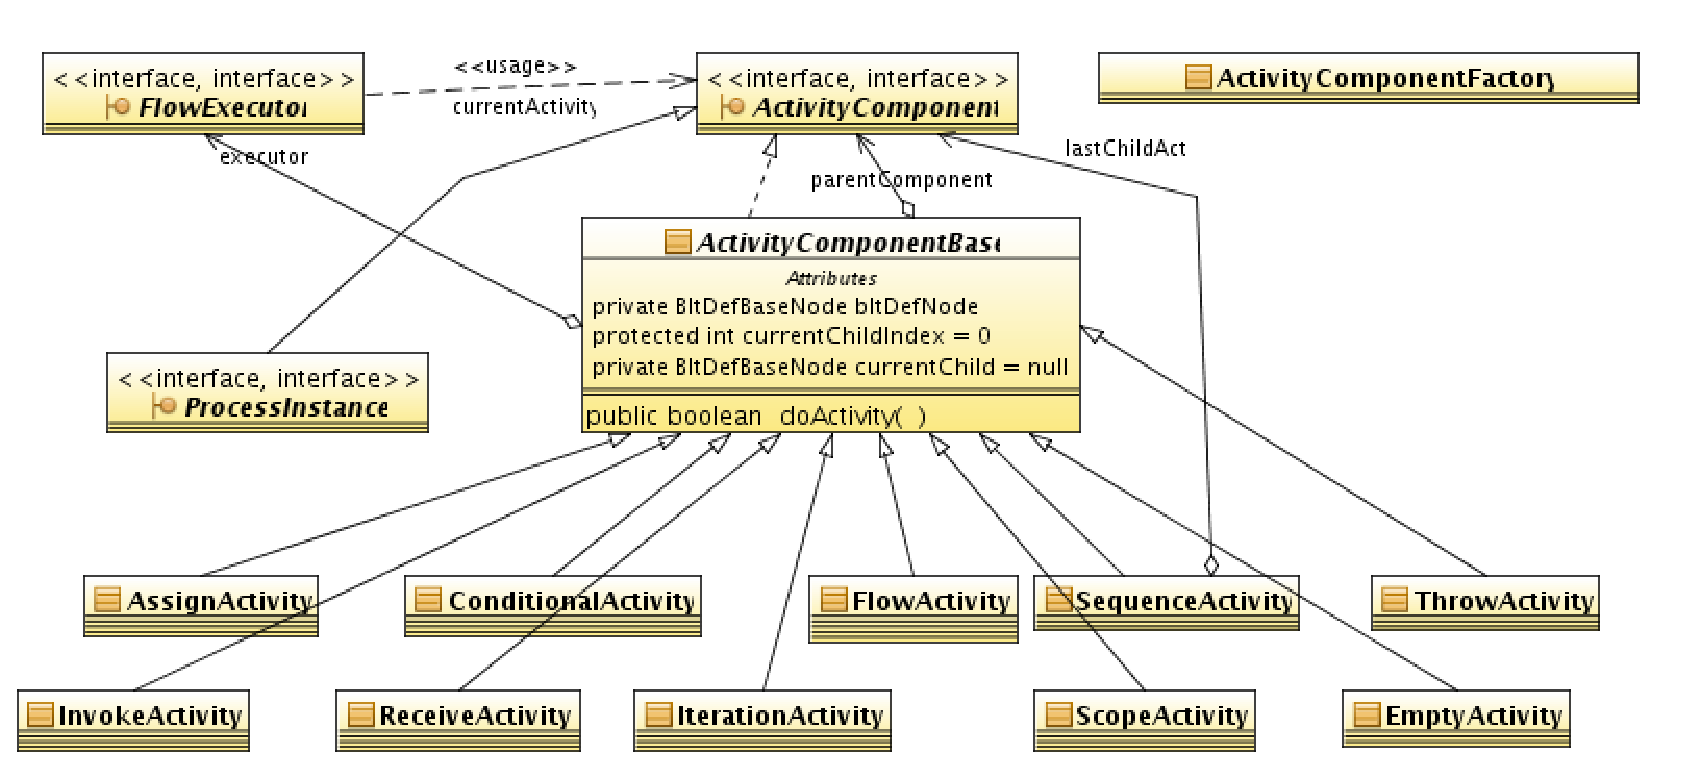
\includegraphics[angle=90,scale=0.80]
{architettura_interna/dia/actclass}
\caption[Gerarchia delle ActivityComponent]{
   	\textsf{{\small Diagramma di classe per la gerarchia delle
   	ActivityComponent}} }
  \label{fig:actclass}
\end{center}
\end{figure}

\section{Esecuzione e parallelismo}

\section{Eventi e comunicazione}
